\chapter{PageRank: Priorisierung im Netzwerk}
\label{chap:pagerank}

\begin{mydefinition}[PageRank]
    PageRank priorisiert Webseiten nicht nur nach der Anzahl eingehender Links,
    sondern auch nach der \textbf{Qualität} dieser Links.
    Eine Seite ist wichtig, wenn wichtige Seiten auf sie verweisen.
\end{mydefinition}

Die Grundidee ist ein \enquote{zufälliger Surfer}:
Mit Wahrscheinlichkeit $d$ folgt er einem Link, mit Wahrscheinlichkeit $1-d$ springt er zufällig auf eine neue Seite.
Der PageRank-Score einer Seite $p$ ist dann:
\[
    PR(p) = \frac{1-d}{N} + d \sum_{q \to p} \frac{PR(q)}{\text{outdeg}(q)}
\]
mit $N$ Seiten und Dämpfungsfaktor $d$ (typisch: $0.85$). Mit outdeg$(q)$ ist die Anzahl ausgehender Links von Seite $q$ gemeint. Mit $PR(q)$ ist der PageRank von Seite $q$ gemeint. Dabei wird $PR(q)$ anfänglich für alle Seiten gleich gesetzt (z.\,B. $1/N$) und iterativ aktualisiert, bis die Werte stabil sind.

\begin{mycaution}
    PageRank ist nicht neutral: Linkfarmen (also Seiten, die sich gegenseitig verlinken), gekaufte Links oder starke Netzwerke können die Rangfolge verzerren.
    Darum braucht man Missbrauchserkennung und zusätzliche Qualitätsmerkmale.
\end{mycaution}

\begin{myexercise}[PageRank intuitiv lesen]
    Betrachten Sie das Netzwerk:
    \begin{itemize}
        \item A verlinkt auf B und C
        \item B verlinkt auf C
        \item C verlinkt auf A
        \item D verlinkt auf C
    \end{itemize}
    Wenn alle Seiten mit gleichem PageRank starten und $d=0.85$ gilt:
    \begin{enumerate}
        \item Welche Seite dürfte nach einem Rechenschritt am höchsten priorisiert sein?
        \item Warum ist ein Link von einer Seite mit vielen Ausgängen weniger wert?
    \end{enumerate}
    \begin{myanswer}
        Nach einem Iterationsschritt ist C am höchsten priorisiert, weil A, B und D auf C verweisen.
        Ein Link von einer Seite mit vielen Ausgängen wird auf viele Ziele verteilt und zählt deshalb weniger stark.
    \end{myanswer}
\end{myexercise}

\begin{myexample}[Berechnung von PageRank]
    Um die PageRank-Werte für die Seiten A, B, C und D aus dem vorherigen Beispiel konkret zu berechnen, kann folgendermassen vorgegangen werden:


    Wir nehmen an, dass $d=0.85$ und setzen die Startwerte alle gleich auf $PR(A)=PR(B)=PR(C)=PR(D)=0.25$. Zunächst stellen wir die Linkstruktur als Matrix dar, wobei die Spalten die Zielseiten und die Zeilen die Quellseiten repräsentieren
    \[
        \begin{array}{c|cccc|c}
                          & A & B & C & D & \text{outdeg} \\
            \hline
            A             & 0 & 1 & 1 & 0 & 2             \\
            B             & 0 & 0 & 1 & 0 & 1             \\
            C             & 1 & 0 & 0 & 0 & 1             \\
            D             & 0 & 0 & 1 & 0 & 1             \\
            \hline
            \text{colsum} & 1 & 1 & 3 & 0 & 4             \\
        \end{array}
    \]
    Nun können wir die PageRank-Werte iterativ berechnen:
    \[
        \begin{aligned}
            PR(A) & = 0.0375 + 0.85 \cdot \left(\frac{PR(C)}{1}\right) = 0.0375 + 0.85 \cdot 0.25 = \underline{0.25}     \\
            PR(B) & = 0.0375 + 0.85 \cdot \left(\frac{PR(A)}{2}\right) = 0.0375 + 0.85 \cdot 0.125 = \underline{0.14375} \\
            PR(C) & = 0.0375 + 0.85 \cdot \left(\frac{PR(A)}{2} + \frac{PR(B)}{1} + \frac{PR(D)}{1}\right)               \\
                  & =0.0375 + 0.85 \cdot (0.125 + 0.25 + 0.25)                                                           \\
                  & =0.0375 + 0.85 \cdot 0.625 = \underline{0.56875}                                                     \\
            PR(D) & = 0.0375 + 0.85 \cdot 0 = \underline{0.0375}
        \end{aligned}
    \]
    Die Korrektheit der oben berechneten Werte kann überprüft werden, indem man die berechneten Werte summiert und sicherstellt, dass sie in etwa 1 ergeben (aufgrund von Rundungsfehlern kann es leicht abweichen). In diesem Fall ergibt die Summe $PR(A) + PR(B) + PR(C) + PR(D) = 0.25 + 0.14375 + 0.56875 + 0.0375 = 1.0$, was bestätigt, dass die Werte korrekt berechnet wurden.

    \cref{fig:pagerank-iterations} illustriert alle iterativen Schritte der Berechnung, beginnend mit den Startwerten und endend mit den stabilen PageRank-Werten. In jeder Grafik sind die Seiten als Knoten dargestellt, wobei die Dicke der Pfeile die Stärke der Verlinkung repräsentiert. Die Zahlen neben den Knoten zeigen die aktuellen PageRank-Werte an, die sich mit jeder Iteration ändern, bis sie stabil bleiben.

    \begin{figure}[H]
        \foreach \step in {00, 01, 02, 03, 04, 05} {
            \begin{subfigure}[H]{0.32\textwidth}
                \centering
                \includegraphics[width=\linewidth]{Grundlagen_Info/10_KI_und_Algorithmen/Figures/pagerank_step_\step.pdf}
                \caption{Iteration \step}
            \end{subfigure}
        }
        \caption{Iterative Berechnung der PageRank-Werte für die Seiten A, B, C und D.}
        \label{fig:pagerank-iterations}
    \end{figure}

    Wie \cref{fig:pagerank-final} zeigt, stabilisieren sich die Werte nach einigen Iterationen, wobei Seite C den höchsten PageRank-Wert von $0.56875$ erreicht, gefolgt von Seite A mit $0.25$, Seite B mit $0.14375$ und Seite D mit $0.0375$. Diese Ergebnisse spiegeln die Struktur des Netzwerks wider, in dem Seite C am meisten verlinkt ist und daher als die wichtigste Seite angesehen wird.

    \begin{figure}[H]
        \centering
        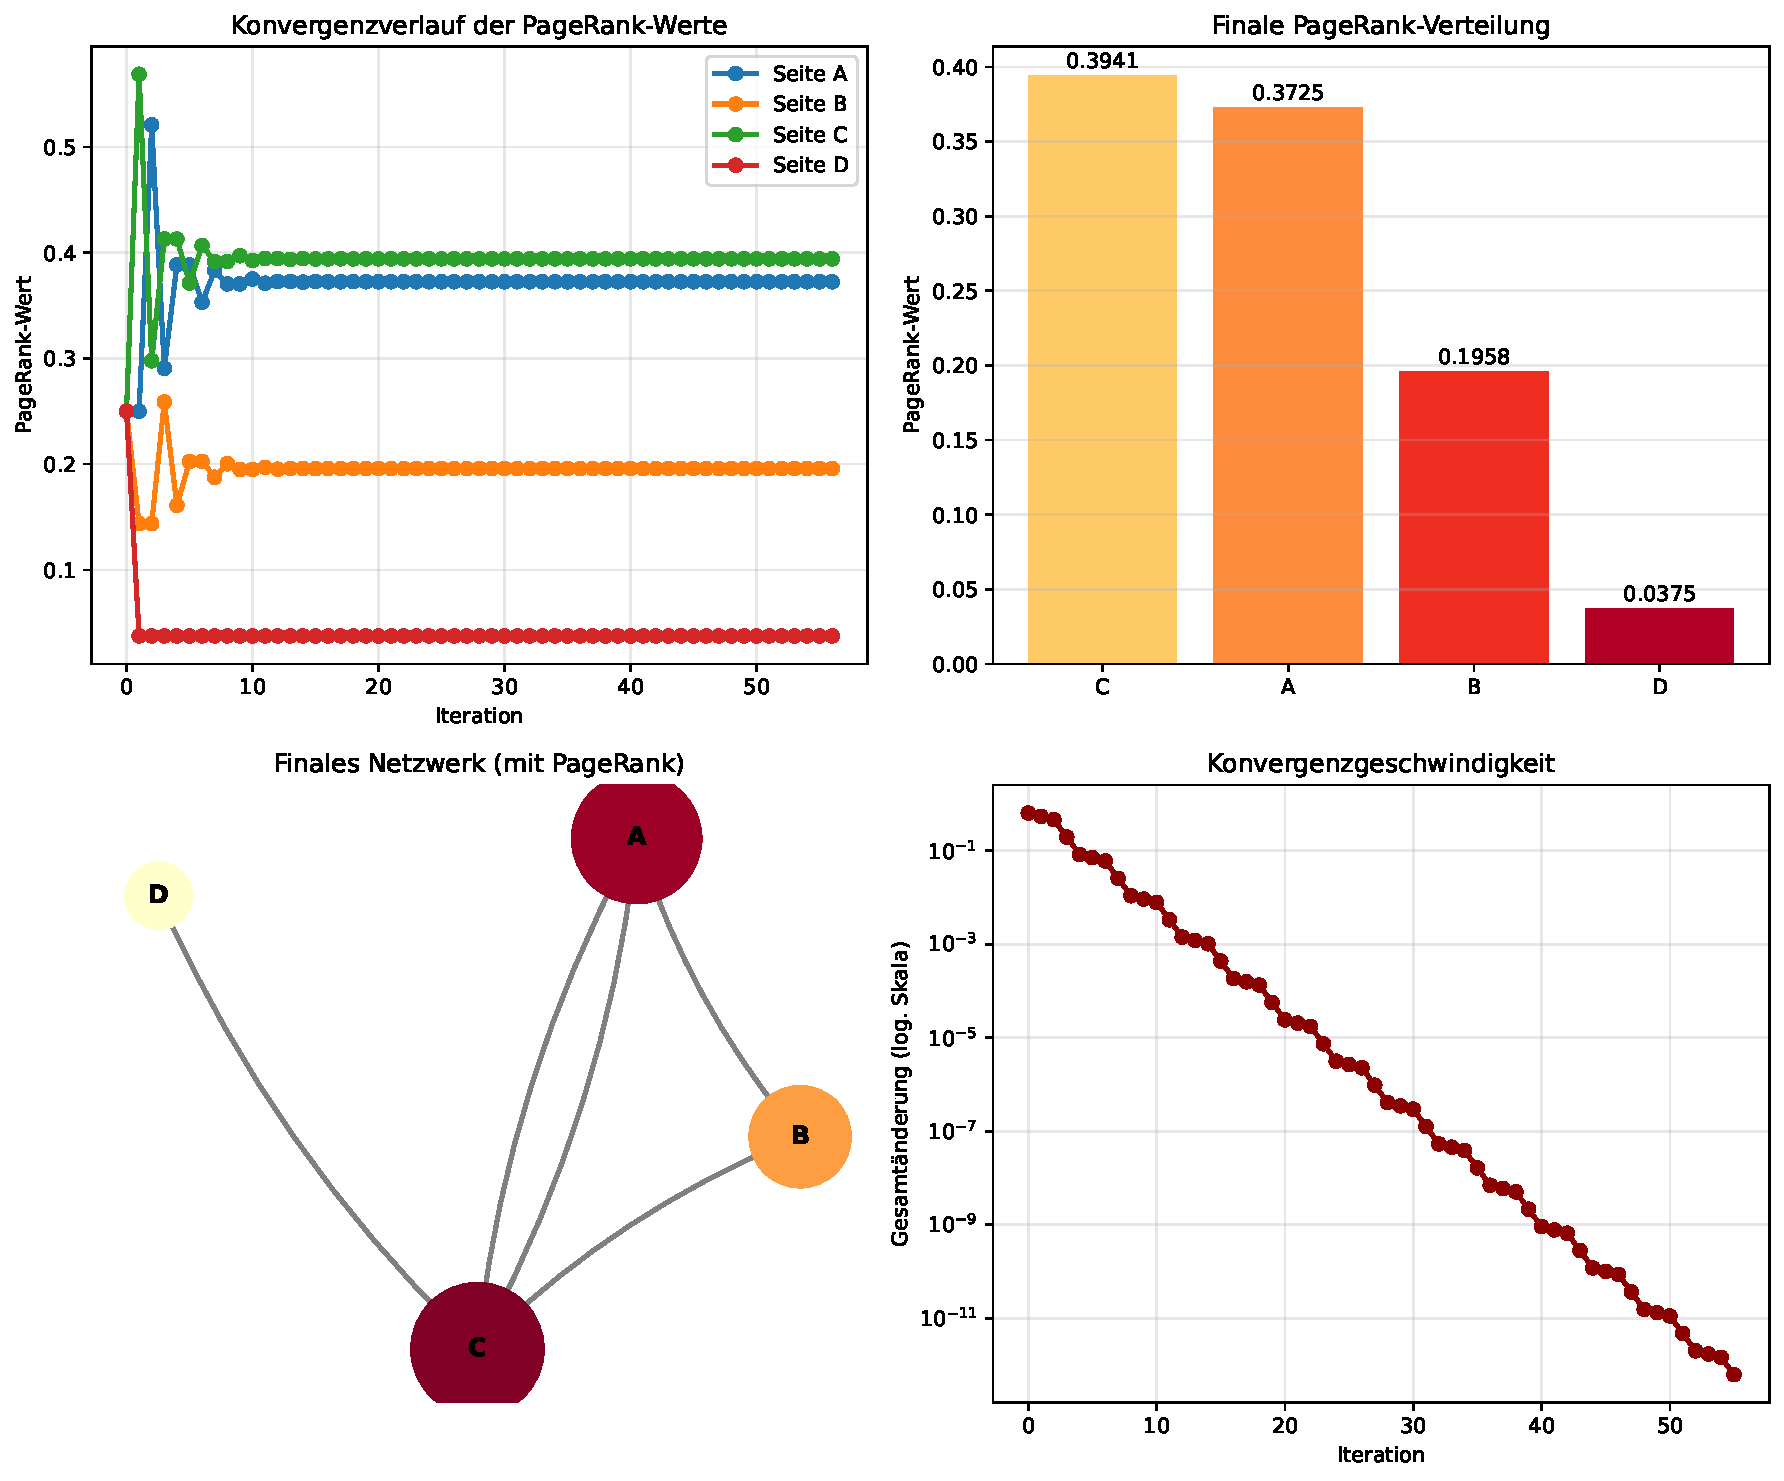
\includegraphics[width=0.8\textwidth]{Grundlagen_Info/10_KI_und_Algorithmen/Figures/pagerank_summary.pdf}
        \caption{Zusammenfassung der finalen PageRank-Werte für die Seiten A, B, C und D.}
        \label{fig:pagerank-final}
    \end{figure}
    
\end{myexample}

\begin{myexercise}[PageRank selber berechnen]
    Sie haben in Ihrem Freundeskreis vier Personen: Alice, Bob, Carol und Dave. Ihre Freundschaften sind wie folgt:
    \begin{itemize}
        \item Alice ist mit Bob und Carol befreundet.
        \item Bob ist mit Alice und Dave befreundet.
        \item Carol ist mit Alice befreundet.
        \item Dave ist mit Bob befreundet.
    \end{itemize}
    Berechnen Sie die PageRank-Werte für jede Person, wenn $d=0.85$ gilt und alle Personen mit einem Startwert von $0.25$ beginnen.

    \begin{myanswer}
    Zunächst stellen wir die Freundschaftsstruktur als Matrix dar:
    \[
        \begin{array}{c|cccc|c}
                          & Alice & Bob & Carol & Dave & \text{outdeg} \\
            \hline
            Alice         & 0     & 1   & 1     & 0    & 2             \\
            Bob           & 1     & 0   & 0     & 1    & 2             \\
            Carol         & 1     & 0   & 0     & 0    & 1             \\
            Dave          & 0     & 1   & 0     & 0    & 1             \\
            \hline
            \text{colsum} & 2     & 2   & 1     & 1    & 6             \\
        \end{array}
    \]
    Nun berechnen wir die PageRank-Werte iterativ:
    \[
    \begin{aligned}
        PR(Alice) & = 0.0375 + 0.85 \cdot \left(\frac{0.25}{2} + \frac{0.25}{1}\right) = 0.0375 + 0.85 \cdot 0.375 = \underline{0.35625} \\
        PR(Bob)   & = 0.0375 + 0.85 \cdot \left(\frac{0.25}{2} + \frac{0.25}{1}\right) = 0.0375 + 0.85 \cdot 0.375 = \underline{0.35625} \\
        PR(Carol) & = 0.0375 + 0.85 \cdot \left(\frac{0.25}{2}\right) = 0.0375 + 0.85 \cdot 0.125 = \underline{0.14375} \\
        PR(Dave)  & = 0.0375 + 0.85 \cdot \left(\frac{0.25}{2}\right) = 0.0375 + 0.85 \cdot 0.125 = \underline{0.14375}
    \end{aligned}
    \]
    Nach einem Iterationsschritt haben Alice und Bob den höchsten PageRank-Wert von $0.35625$, gefolgt von Carol und Dave mit jeweils $0.14375$. Die PageRank-Werte summieren sich auf $0.35625 + 0.35625 + 0.14375 + 0.14375 = 1.0$.
    \end{myanswer}
\end{myexercise}

\begin{mychallenge}[Priorisierung vergleichen]
    Vergleichen Sie gewichtete Priorisierung und PageRank:
    \begin{enumerate}
        \item Welche Methode ist leichter erklärbar?
        \item Welche Methode ist anfälliger für Manipulation?
        \item Wo würden Sie welche Methode im Schulkontext einsetzen?
    \end{enumerate}
\end{mychallenge}

\begin{myremark}[Notebook]
    Praktische Umsetzung inkl. Übungen:
    \href{\notebookurl}{\texttt{10\_KI\_und\_Algorithmen/06\_Priorisierung\_PageRank.ipynb}}
\end{myremark}

\cref{ch:pagerank-markov} zeigt, wie PageRank als stationäre Verteilung einer Markov-Kette interpretiert werden kann, was die mathematische Grundlage für die Berechnung von PageRank bildet. Dort wird auch ein konkretes Beispiel durchgerechnet, um die Verbindung zwischen der Linkstruktur eines Netzwerks und den resultierenden PageRank-Werten zu verdeutlichen.

\begin{mychallenge}[PageRank als Markov-Kette in Pythonumsetzen]
Lesen Sie \cref{ch:pagerank-markov} und setzen Sie den PageRank-Algorithmus als Markov-Kette in Python um.
\end{mychallenge}
